\documentclass{article} 
\usepackage{apacite} 
\usepackage{graphicx} 
\usepackage{natbib}
\usepackage{listings}
\usepackage{epigraph} 
\usepackage{etoolbox} 
\usepackage{amsmath}

\usepackage{color}
\usepackage{array}
\newcolumntype{L}[1]{>{\raggedright\let\newline\\\arraybackslash\hspace{0pt}}m{#1}}

\definecolor{Red}{RGB}{255,0,0}
\newcommand{\red}[1]{\textcolor{Red}{#1}}  
  
\usepackage{listings}
%\usepackage{inconsolata}
\usepackage{xcolor} %to use colored text

%\lstset{
%language=Scheme,\lstinline
%basicstyle=\footnotesize\ttfamily,
%mathescape=true,
%frame=single
%}

\lstset{
  language=Scheme, % Andreas Stuhlmüller. Scheme listings. https://github.com/stuhlmueller/scheme-listings.git
  columns=fixed,
  tabsize=2,
  extendedchars=true,
  breaklines=true,
  frame=single,
%  numbers=left,
  numbersep=5pt,
    basicstyle=\scriptsize\ttfamily
%  rulesepcolor=\color{solarized@base03},
%  numberstyle=\tiny\color{solarized@base01},
%  keywordstyle=\color{solarized@green},
%  stringstyle=\color{solarized@cyan}\ttfamily,
%  identifierstyle=\color{blue},
%  commentstyle=\color{solarized@base01},
%  emphstyle=\color{solarized@red}
}

\makeatletter
\patchcmd{\epigraph}{\@epitext{#1}}{\itshape\@epitext{#1}}{}{}
\makeatother \def\signed
#1{{\leavevmode\unskip\nobreak\hfil\penalty50\hskip2em
\hbox{}\nobreak\hfil#1% \parfillskip=0pt \finalhyphendemerits=0
\endgraf}} \newsavebox\mybox \newenvironment{aquote}[1]
{\savebox\mybox{#1}\begin{quote}} {\signed{\usebox\mybox}\end{quote}}
\DeclareGraphicsExtensions{.pdf,.png,.jpg}
% Default margins are too wide all the way around. I reset them here
\setlength{\topmargin}{-.5in} \setlength{\textheight}{9in}
\setlength{\oddsidemargin}{.125in} \setlength{\textwidth}{6in}

\begin{document} \title{Motivated reasoning in minimal groups}
\author{Erik Brockbank, Andres Gomez Emilsson, and Michael Henry Tessler} \renewcommand{\today}{Psych 241\\June 8,
2014} \maketitle

\section{Introduction}

\subsection{Motivated reasoning}

\subsection{Sources of motivated reasoning: optimism biases}

\section{Minimal groups}

\section{Two computational models}

We compose a generative model that considers an team game analogous to that used in \citet{Klein1992}. A game is made up of two teams playing in parallel to accrue points. A point in the game is a Bernoulli random variable that can be true in one of two ways: either by the team being skillful or by the team being lucky, as in:

\begin{lstlisting}
   (define (single-hit team type-of-game)
    (if (flip (luck type-of-game)) 
      (flip) 
      (flip (team-ability team))))
\end{lstlisting}

A team gets lucky according to probability 0.5 in situations where the point is determined by luck, this latter component is determined by \lstinline{(flip (luck type-of-game))}. This captures the intuition that some games have a lot of luck involved, whereas others are determined largely by chance. If the round is not determined by luck, then the team gets a hit in proportion to their teams abilities. 

Our game involves teams with distinct roles and as such, the \lstinline{team-ability} could be determined by the product of the individual players' abilities, as in:

\begin{lstlisting}
   (define (team-ability team)
     (prod (map (lambda (person) (player-ability person)) team)))
\end{lstlisting}

However, in the \citet{Klein1992} setup, as well as in ours below, there is reason to believe the roles are asymmetric. As well, using the product of the two players abilities to determine the probability of a correct answer makes the task more difficult than we would expect. This is important when we consider inferences about \lstinline{luck} later. For these reasons, our models consider the team's ability to be determined by only one player, as in:

\begin{lstlisting}
(define (team-ability team) (strength (first team)))
\end{lstlisting}

We consider a player's ability to a persistent, but random, property of the individual. We consider the luck in a game to be defined similarly. 

\begin{lstlisting}
   (define player-ability (mem (lambda (person) (ability-prior))))
   (define luck (mem (lambda (type-of-game) (luck-prior))))
\end{lstlisting}

As a first pass, we define \lstinline{ability-prior} and \lstinline{luck-prior} to be drawn from a \lstinline{(beta 5 5)} distribution. 

In \citet{Klein1992}, participants were given evidence about the past performance of a target individual. The evidence they received was in the form of \lstinline{total-hits}, which is defined as \lstinline{(repeat num-rounds (lambda ()   (single-hit team type-of-game)))}. Thus, the form of the evidence the participants received was 

\begin{lstlisting}
(condition (equal? (total-hits '(target other) 'history 8) 8))
\end{lstlisting}

This says that the total-hits of the target person in an game which had eight rounds was equal to 8. The reason \lstinline{'other} is included is because the game is a two-person game, and so even though the other player is not referred to explicitly in the evidence, she needs to be included to make sense of the \lstinline{total-hits} function. Notice also that the string \lstinline{'history} is used to signify that we are referring to a particular type of game (e.g. the history game). This is important in determining the value of \lstinline{(luck type-of-game)}, which we defined as a persistent property of a game.

The predictions of the base model in Figure \ref{fig:base}. Throughout this modeling section, we will show plots with bootstrapped 95\% confidence intervals for the following four quantities: (1) perceived ability of target (2) perceived ability of the average player (or, a randomly selected new player) (3) perceived luck in the game and (4) the probability of winning a game against a team that includes the target individual. 

\begin{figure}
\centering
    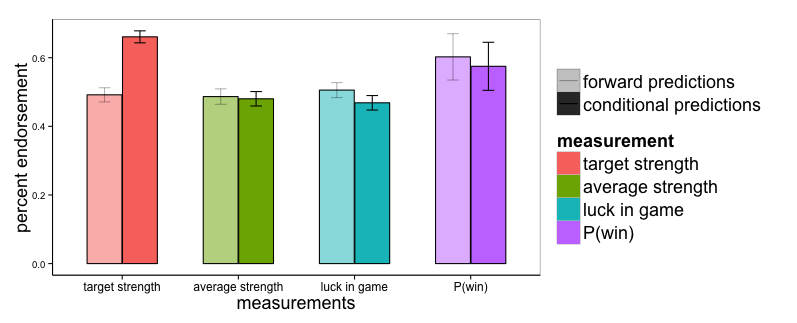
\includegraphics[width=\columnwidth]{basePredictions2}
    \caption{Base model predictions. The forward predictions are simply the results of the generative model conditioned on no evidence. The conditional predictions are those conditioned on the target getting 8 out of 8 questions correct on the previous round.}
      \label{fig:base}
\end{figure}


Below, we consider two possible sources of motivated reasoning: optimism and perceived excellence. 
\subsection{Optimism model}

In the Optimism model (henceforth, Model O), the participant is optimistic about his expected performance in the upcoming match. This is operationalized in the model by introducing a new conditioning statement: 

\begin{lstlisting}
      (if (flip optimism) 
        (eq? 'team1 (match-winner my-team their-team game num-rounds)) 
        (eq? 'team2 (match-winner my-team their-team game num-rounds)))
\end{lstlisting}

This states with with a certain degree of optimism \lstinline{(flip optimism)}, the participant expects her team will win the next match. If \lstinline{optimism} is equal to 1, the state of the world is updated as if the participant has already won. If  \lstinline{optimism} is equal to 0, the participant believes with absolute certainty that she will lose. To account for the effects of \citet{Klein1992}, \lstinline{optimism} would fall between 0.5 and 1. 


\subsection{Excellence model}
In the Excellence model (model E), the participant does not have optimistic (or pessimistic) expectations about the future but rather believes she is an above average player. This would also lead to a ``better than expected" performance at the game (meaning that the probability that her team will win is better than the evidence would suggest). For this we need to assume that the participant is uncertain about what the average ability is (or, equivalently, how difficult the game is), but knows that whatever the average is, she is better than it.

The influence on the experimental queries is a little more subtle in this model. 

\section{Experiment 1}

\subsection{Methods}

Both Experiment 1 and Experiment 2 attempt to replicate in an online setting the empirical results observed in Klein and Kunda (1992). The general structure of the experiment will be outlined here, and in the Experiment 2 section the improvements made upon Experiment 1 will be discussed.

According to the literature reviewed, motivated reasonig manifests in the difference in skill level attributed to a player (who we call DW) that is judged based on previous performance. When the study participant wonders about DW's strength at a game, his beliefs could be influenced by what is at stake in the game. Since both the relationship between the person being judged and the information available about that person seem to matter for motivated reasoning, our study incorporates a 2x3 condition design with a conpetition condition and an evidence condition. The competition condition describes the relationship between the study participant and DW, who is either a partner (P), an opponent(O), or a control (C, who is neither a partner nor an opponent). Motivated reasoning anticipates that DW will be judged as having a highest ability in the Partner condition, the lowest ability in the Opponent condition, and in-between when DW in the control condition. 

Mirroring the conditons of Klein and Kunda (1992), we employed two evidence conditions. These conditions are called the high and the low evidence condition and they determine the amount of information provided about DW. As a cover story, we tell participants that we will show them the performance of

Since the effect is set to happen before the actual game is played, the study does not require putting particpants in touch with each other.

\subsection{Materials}

We hosted the website at http://langcog.stanford.edu/expts/index-clean.html, and linked to it from Amazong Mechanical Turk (AMT) so that participant could navigate an embeded verion of our experiment in the very webpage they accepted to participate in the study. We recruited 145 AMT participants. Each participant was compensated with 25 cents for their participation, and one fourth of the participants were selected randomly and were awarded with a \$1 bonus (which will be explained below).

Of the 145 subjects, we excluded 20 from the analysis due to failing the competition condition manipulation check. These are participants that failed to recognize their relationship with DW (e.g. someone stating that DW is his opponent when DW had been assigned as a partner).


\subsection{Procedure}

Each participant is assigned to a competition condition and to an evidence condition at random (with equal probabily for each of the permutations). Before they accept to participate, participants are told that the task will take less than 10 minutes (which is the maximum time allocated to complete the task), that they will be compensated with 25 cents for participating (and that they can leave the study anytime if they so desire). Once they accept to particpate, we ask them to write down their initials (e.g. AGE) and we explain to them that they are about to play two rounds of a \"word game\" with a live partner. The game consists of two teams, each consisting of two persons: a word selector and a word unscrambler. The precise wording is:

``Each team will have a word selector and a word unscrambler. The word selector will select a word from a list of 6-letter words. The word will appear scrambled, and the word unscrambler will have 10 seconds to figure out the original word. Each team will repeat this process for ten words, and the team with the greater number of correct answers could earn up to 1 dollar, depending on the margin of difference between the two teams."

Stating that they can earn up to 1 extra dollar if they win the game is intended to enhance the outcome dependency of the study, to increase motivation and thus enhance the potential for motivated reasoning. 

To enhance the believability of the setting, we display a dynamic \"waiting\" gif for 20 seconds while the server is \"finding players,\" followed by a 4 second wait to \"load the game.\" As a cover story to present participants with evidence about DW's previous performance, we tell them that we will show them the results from a previous round in order for them to become familiar with the game. We then show DW's previous unscrambling performance by asking them to click a \"continue button\" either 2 or 8 times (depending on the evidence conditon). Each time we reveal a scrambled word, the correct unscrambled word and whether or not DW answered correctly. In this study, all the words were 6 letter words, ranging from easy (banana) to extremelly challenging (schism). All participants saw that DW answered each question correctly.

In the followig slide participants were asked to rate DW's \"unscrambling ability\", the average ability of other Turkers (the people who do AMT tasks), the perceived \"role of luck in the game\" and the probability that their team will win. Next, a slide containing manipulation checks (e.g. \"Is DW a parter, opponent, or neither?\") and an open text field to enter open ended comments (which was intended to detect whether participants believed that they were going to play against a real human being).


Participants were then fully debrief, and an open text field was provided for final comments about the experiment. 




\subsection{Results}

%Show: motiv-facetQuestion_mht0_n140-lines.png, or motiv-facetQuestion_mht0_n140.png.

We used an anova test to analyze what accounts for the variance of the estimated strength DW. The evidence condition is significant at the p < 0.001 level, but the competition condition is not significant. When an interaction between the conditions is tested, the result is that only the evidence condition remains significant (and not the interaction variable). When other vairables are included as predictors, such as the average strength of AMT participants, the role of luck in the game and the expectation of winning, the competition condition remains non-significant. A statistical sigificance of the competition condition as a predictor for DW strenght was not found in any further analysis.

As it can be seen in (DW_strength_pilot.png), the mode of DW's strength as estimated by the participants is the highest possible value. Clearly the items were regarded as considerably harder than what people are capable of unscrambling in the time provided. We call this a ceiling effect, where the scale becomes less useful due to an extreme skewing of the possible answers. Numerically, the average DW strength is for the high evidence condition is 0.8798980 (0.8435525, 0.9101150, 95\% bootstrapped confidence intervals), and 0.7799735 (0.7516508, 0.8099752, 95\% bootstrapped confidence intervals).

\section{Experiment 2}

\subsection{Methods}


Since we did not find evidence of motivated reasoning in this study, we proceeded to make some changess for Experiment 2 to increase the likelihood of a non-null result. This experiment is an improvement upon Experiment 1 in various ways. First, a sense of \"team affiliation\" was cultivated throughout the experiment by making who is on which team much more salient. To do that large banners that represent each team were displayed when teams were assigned. The teams were called \"Red Team\" and \"Blue Team\" and it was made very explicity that the participant was in the red team with another person. 

In addition the visual guide, a small \"chat box\" was designed to appear to be a comunication channel between the participant and their partner. Automatically the box would first display: \"SK: ... (typing)\" quickly followed by \"SK: We can do this!\" to create the illusion that the participant's partner is a real person involved in the task and motivated to win. See team_picture.pmg.

Additionally, the difficulty of unscrambling words was conveyed more realistically: By making participants engage in three practice unscrambling questions right before they were presented with DW's past performance. This in turn was also displayed in a more compelling way than in Experiment 1, showing additional information like the number of seconds that DW took to answer the question.

Since a ceiling effect for DW's strength was found in Experiment 1, the evidence was tweaked to maximize the level of ambiguity about DW's actual ability to unscramble words. Only one evidence condition was used: two questions, out of which only the easier one was solved by DW.

\subsection{Materials}

We recruited 88 participants from AMT. Those who did not pass the competition condition manipulation check were excluded from the analysis, leaving 63 compliant participants.

\subsection{Procedure}

Same as for Experiment 1 except for the changes outlined in the Methods section. The input from the participant was slightly modified: In addition to role of luck, probability of winning, etc. participants were also asked to rate \"how motivated they were to win.\" Finally, particpants were asked to provide their age, gender, and their first language. 

\subsection{Results}

Show: motiv2_facet-Question_n48.png

Similarly to what was found in Experiment 1, ANOVA analysis showed that the competition condition was not significantly different between the competition conditions. A t-test did not show a statistically significant difference between the conditions. Controlling for other variables such as age, gender, first language and other elements asked about such as role of luck in the game and the strength of the average Turker.


\section{Discussion}


Notice that the potential gain in this study is substantially smaller than the potential gain in the original face-to-face version (where the possible bonus for winning was \$50 dollars). This figure needs to be considered in context; the mean participant remuneration is in fact-to-face studies is typically larger than similar online studies by one or two orders of magnitude. Thus, while the absolute value of the possible bonuses is very different, the relative value of the bonuses compared to the standard awards for participation are approximately the same. 

In light of the null results, it is worth examining whether motivated reasoning arises in a manner that depends on the available gains in a given context, or if the phenomenon requires a significance above certain absolute value (e.g. \$20). First, it could be that the small possible bonus (\$1) fails to arise a sufficiently high degree of motivation in the participants for the effect to be elicited. The problem with this view is that the mean self-reported \"motivation to win\" in the compliant participants of the second study is 0.8402576 (+0.04730962, -0.05015323, 95\% bootstrapped confidence interval) and a large minority even chose the ceiling value (1). To confirm that the \$1 bonus is responsible for an enhanced motivation might be investigated in the future. Second, perhaps the self-reported motivaiton is not truely representative of the kind of motivation that leads to motivated reasoning. If this is so, then it would be worth considering alternative ways to measure motivation (such as perseverance in the face of technical problems).

Another possible explanation for the null result would be that participants did not fully understand one or more aspects of the study. In Study 2 participants reported being native English speakers without exception. Thus, while we did not ask about participant's first language in Study 1, we are confident that non-native English speakers are not the cause of the null result. Likewise, the number of people who failed to remember how many questions were displayed during familiarization and how many of them were answered correctly by DW is about 4 out of 5 in both studies. Excluding participants who did not satisfy this criteria from the analysis does not return significant results either. 

Finally, it could be that the evidence provided does not allow participants to construct a believable and desirable account of DW's strength in more than one way. As argued in Klein and Kunda (1992), motivated reasoning arises only when people have information at their disposal with which to construct justifications for one's desired beliefs. The evidence that we presented participants in Study 1 was very similar to the evidence used in the original study. I.e. two or eight questions, all answered correctly. We obtained a ceiling effect and hypothezised that it could account for the null result, but it is not clear that the original study did not also have a ceiling effect (with means ranging from 6.4 to 8.1 out of 10). Even with the ceiling effect we obtained, we still saw a statistically significant difference for the evidence condition. More so, we obtained a wide spread of estimated DW strengths in Study 2 (mean of 0.57, sd of 0.197). Thus the ceiling effect is not a plausible explanation for the null results. The remaining point could be that the subject matter and difficulty of the questions we used simply do not lend themselves to motivated reasoning. Perhaps people can more readily justify their belief about a person's knowledge of American History, but cannot make a plausible story to justify motivated beliefs about ability to solve anagrams. 

\bibliographystyle{apacite}

\setlength{\bibleftmargin}{.125in}
\setlength{\bibindent}{-\bibleftmargin}

\bibliography{motivation}

\end{document}
